\chapter{Access to the VSC Cloud}
Access to the VSC Cloud is linked to the central VSC account system
(\href{https://account.vscentrum.be}{account.vscentrum.be}), so you do
not need a separate login or password.  In order to use the cloud
services,
\begin{itemize}
\item you need an active VSC account and
\item your account must be a member of one or more OpenStack projects.
\end{itemize}
New users can obtain an account by following
\href{https://vlaams-supercomputing-centrum-vscdocumentation.readthedocs-hosted.com/en/latest/access/account_request.html}{the
  procedure described here}.  Once you have an account, contact
\cloudinfo if you want to start a new OpenStack project, or join an
existing one.

You can interact with the VSC Cloud using the OpenStack Dashboard, a
web interface, or the OpenStack command line interface, which you can
use from any system, and which is installed for you on the UGent login
node \lstinline{login.hpc.ugent.be}.  You can log in to the Dashboard
using the VSC accountpage, as illustrated in the next section.  To get
access from the command line interface, you'll need to obtain an
application credential, as explained in section \ref{sec:appl-cred}.

These restrictions do not apply to someone who simply wishes to access
an existing VM running in the cloud.  VSC Cloud projects can decide
themselves who gets access to their VM's, and how.

\section{Dashboard Login}\label{sec:dashboard-login}
You can access the OpenStack web interface, or Dashboard, via \href{https://cloud.vscentrum.be}{cloud.vscentrum.be}.

To log in, choose the (default) authentication method \emph{VSC Accountpage} and click \strong{Connect}.
\begin{center}
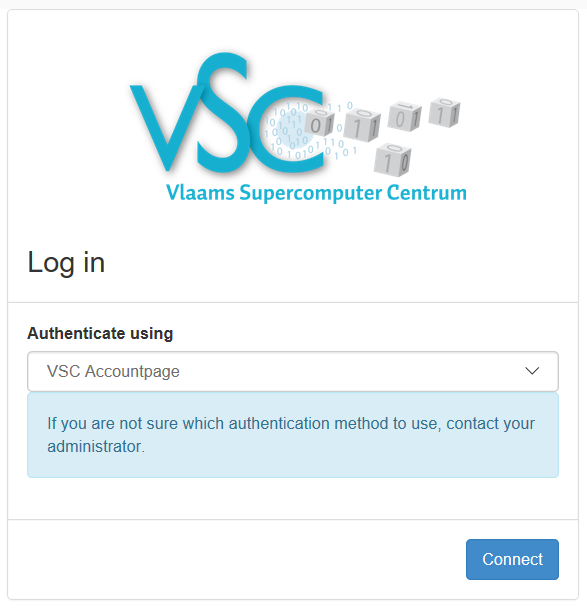
\includegraphics[width=0.5\textwidth]{img/cloud_login_1.png}
\end{center}

From here on, follow the standard procedure to log in to your VSC
account, using your home institution's single sign-on system.  You can
find a detailed description in the HPC introduction at
\href{https://hpcugent.github.io/vsc\_user\_docs}{hpcugent.github.io/vsc\_user\_docs}.
The following chapters explain how to accomplish basic tasks using the Dashboard.

\section{Application Credentials}\label{sec:appl-cred}
If you want to use the OpenStack command line interface  --- or, for advanced users, use the OpenStack APIs directly --- you need to identify yourself using an application credential.  An application credential contains a secret piece of information which grants access to an OpenStack project on your behalf.

You can create an application credential using the dashboard:
\begin{enumerate}
\item Log in to the dashboard, and, if you are a member of more than
  one project, select the project for which you want to create an
  application credential.
\item Open the \textbf{Identity} tab, and click \textbf{Application
    Credentials}.
\item You can now see an overview of your application credentials
  (initially none).  Click \textbf{Create Application Credential}.
\item Fill out the \textbf{Create Application Credential} dialog:
  \begin{description}
  \item[Name, Description] Choose a name (mandatory) and description
    that remind you of the purpose of this credential.
  \item[Secret] We recommend to leave this empty, in which case
    OpenStack will generate a random secret for you.
  \item[Expiration Date, Expiration Time] It is good practice make the
    token expire.  An expiration date limits the impact if the secret
    is accidentally exposed, and you can always create a new
    credential when an old one is expired.
  \item[Roles] A role defines a set of access rights. By selecting a
    subset of roles for this credential, you can limit the access
    rights granted by this credential.  It is a good idea to select
    only the minimal set of roles required for the task you want to
    accomplish.
  \end{description}
  Click \textbf{Create Application Credential}.
\item A summary dialog with the credential's id, name, and secret is
  displayed.  If you close the window, you can't retrieve the secret
  anymore, so you should save it now.  A convenient solution is to
  download the openrc file, a shell script that sets the appropriate
  environment variables for the command line interface.
\end{enumerate}

The newly created credential is now shown in the overview.  If you
accidentally expose a credential somewhere, you should delete it here
to prevent unauthorized access to the system.

%%% Local Variables:
%%% mode: latex
%%% TeX-master: "intro-Cloud"
%%% End:
